\documentclass{beamer}
\mode<presentation> {
\usepackage{verbatim}

\usetheme{Madrid}
\usepackage{xcolor}
\usepackage{caption}
\usepackage{graphicx}
\usepackage{caption}
\usepackage{subcaption}
\usepackage{eqnarray,amsmath}
\usepackage{multirow}
\usepackage{MnSymbol}
\usepackage[utf8]{inputenc}
\usepackage{listings}
\usepackage{color}
\usepackage{graphicx}
\usepackage{sidecap}

\usepackage{pgf}
\usepackage{tikz}



\DeclareCaptionFont{white}{\color{white}}
\DeclareCaptionFormat{listing}{%
	\parbox{\textwidth}{\colorbox{gray}{\parbox{\textwidth}{#1#2#3}}\vskip-4pt}}
\captionsetup[lstlisting]{format=listing,labelfont=white,textfont=white}
\lstset{frame=lrb,xleftmargin=\fboxsep,xrightmargin=-\fboxsep}
\usetikzlibrary{arrows,automata}
\usetikzlibrary{positioning}

\lstset{escapeinside={<@}{@>}}
\tikzset{
	state/.style={
		rectangle,
		rounded corners,
		draw=black, very thick,
		minimum height=2em,
		inner sep=2pt,
		text centered,
	},
}
\setbeamertemplate{caption}[numbered]

\newcommand{\mat}[1]{${#1}$}
\newcommand{\bb}[1]{{\texttt{B#1}}}
\newcommand{\R}{\texttt{R}}
\newcommand{\W}{\texttt{W}}
\newcommand{\RW}{\texttt{RW}}
\newcommand{\X}{\texttt{X}}
\newcommand{\RWX}{\texttt{[R,W,RW]}}
\newcommand{\CPU}{\texttt{CPU}}
\newcommand{\GPU}{\texttt{GPU}}
\newcommand{\CG}{\texttt{[CPU,GPU,X]}}
\newcommand{\atup}[1]{\texttt{({#1})}}
\newcommand{\egen}[1]{$GEN[#1]$}
\newcommand{\ekill}[1]{$KILL[#1]$}
\newcommand{\ein}[1]{$IN[#1]$}
\newcommand{\eout}[1]{$OUT[#1]$}
\newcommand{\ca}[1]{\ttt{CA = #1}}

\newcommand{\etal}{{\em et al. }}
\newcommand{\cL}{{\cal L}}
\newcommand{\map}{\texttt{map} }
\newcommand{\unmap}{\texttt{unmap} }
\newcommand{\rb}{\texttt{readBuffer} }
\newcommand{\rcap}[1]{Chapter~\ref{cap:#1}}
\newcommand{\rsec}[1]{Section~\ref{sec:#1}}
\newcommand{\rsecs}[2]{Sections~\ref{sec:#1} --~\ref{sec:#2}}
\newcommand{\rtab}[1]{Table~\ref{tab:#1}}
\newcommand{\rfig}[1]{Figure~\ref{fig:#1}}
\newcommand{\rfigs}[2]{Figures~\ref{fig:#1} --~\ref{fig:#2}}
\newcommand{\rlst}[1]{Listing~\ref{lst:#1}}
\newcommand{\req}[1]{Equation~\ref{eq:#1}}
\newcommand{\reqs}[2]{Equations~\ref{eq:#1} --~\ref{eq:#2}}
\newcommand{\ttt}[1]{{\texttt{#1}}}
\newcommand{\tit}[1]{{\textit{#1}}}

}
\RequirePackage[utf8]{inputenc}
\usepackage[english]{babel}
%\usepackage[latin1]{inputenc}
\title[Master Defense]{\textbf{Support for Parallel Scan in OpenMP}}
\author{\textbf{E. Maicol G. Zegarra}}
\institute[LSC-IC/UNICAMP] 
{
\textit{maicol.zegarra@students.ic.unicamp.br}\\
University of Campinas \\
Institute of Computing\\
\medskip
\flushright {Advisor\\Prof. Dr. Guido Costa Souza de Araújo}\\
\flushright {Co-advisor\\Prof. Dr. Marcio Machado Pereira}\\
\centering
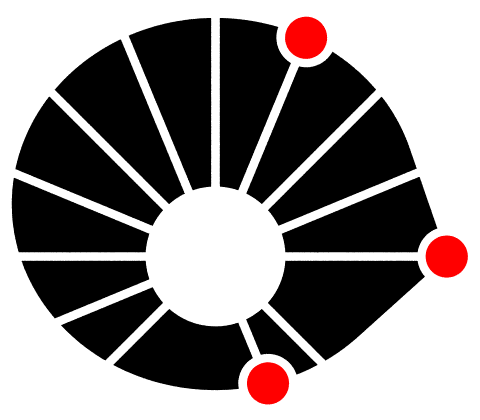
\includegraphics[scale=0.1]{unicamp.png} \hspace*{1.0cm}~%
   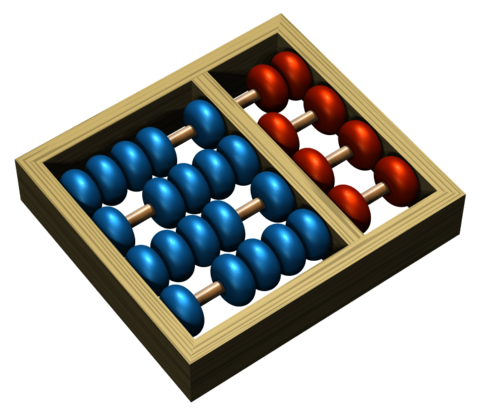
\includegraphics[scale=0.1]{ic.png}
}

\date{24 April 2018} 
\begin{document}

%*******************Contents*******************

\frame{\titlepage}
\begin{frame}
\frametitle[]{\textbf{Table of Contents}}
\tableofcontents 
\end{frame}

%*******************Introduction*******************
\section{Introduction}

\begin{frame}
	\frametitle{\textbf{Table of Contents}}
	\tableofcontents[currentsection]
\end{frame}

\frame{
	\frametitle{\textbf{Parallel Quicksort Algorithm}}
	\begin{figure}[]
		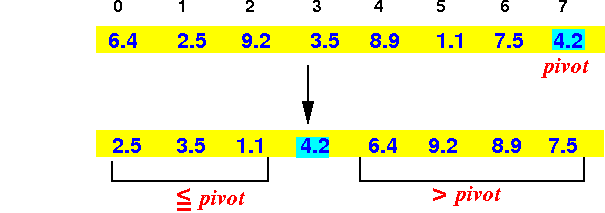
\includegraphics[width=9cm,height=3.5cm]{Figures/quicksort.png}
	\end{figure}
	How can we do this in parallel?
}

\frame{
\frametitle{\textbf{Prefix Sums Problem}}

In computer science, the prefix sum, cumulative sum,\\inclusive scan or simply scan is defined as:\\
\begin{itemize}
	\item Given a \textbf{binary associative operator} $\oplus$;
	\item An ordered set of $n$ elements [$a_{0}$, $a_{1}$, ... , $a_{n-1}$];
	\item Return the ordered set [$a_{0}$, $a_{0}$ $\oplus$ $a_{1}$, ... , $a_{0}$ $\oplus$ $a_{1}$ $\oplus$ ... $\oplus$ $a_{n-1}$].
\end{itemize}
}

\frame{
\frametitle{\textbf{Prefix Sums Problem}}
There are two versions of Prefix Scan: inclusive and exclusive. \\
\begin{figure}[]
	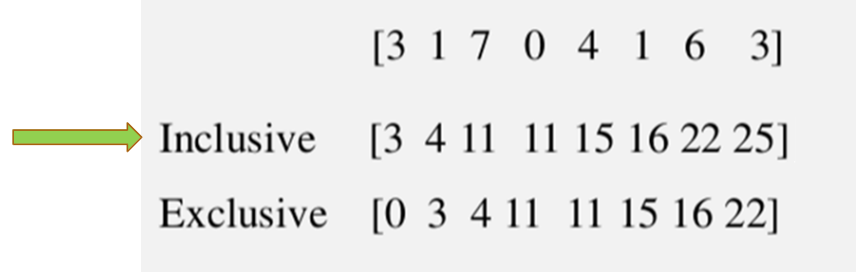
\includegraphics[width=9cm,height=2.5cm]{Figures/inclusive_exclusive.png}
\end{figure} 
}

\frame{
	\frametitle{\textbf{Prefix Sums Problem}}
	There are two versions of Prefix Scan: inclusive and exclusive. \\
	\begin{figure}[]
		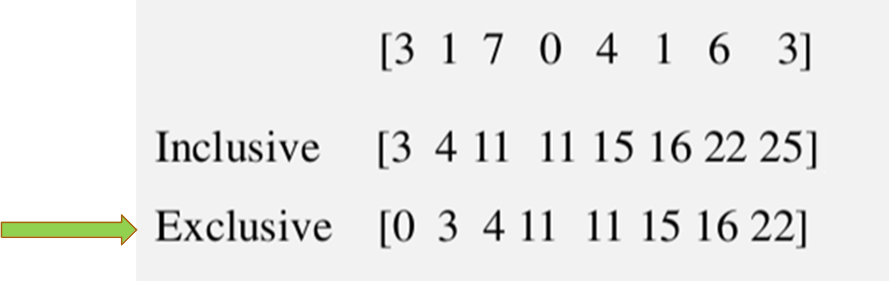
\includegraphics[width=9cm,height=2.5cm]{Figures/inclusive_exclusive_2.png}
	\end{figure} 
}

%------------------The Algorithm---------------------
\section{The Algorithm}

\begin{frame}
	\frametitle{\textbf{Table of Contents}}
	\tableofcontents[currentsection]
\end{frame}


\frame{
	\frametitle{\textbf{Algorithm (Proposed by Horn in 2005 )}}
	Based in Hillis and Steele Work (1986).
	\begin{figure}[]
		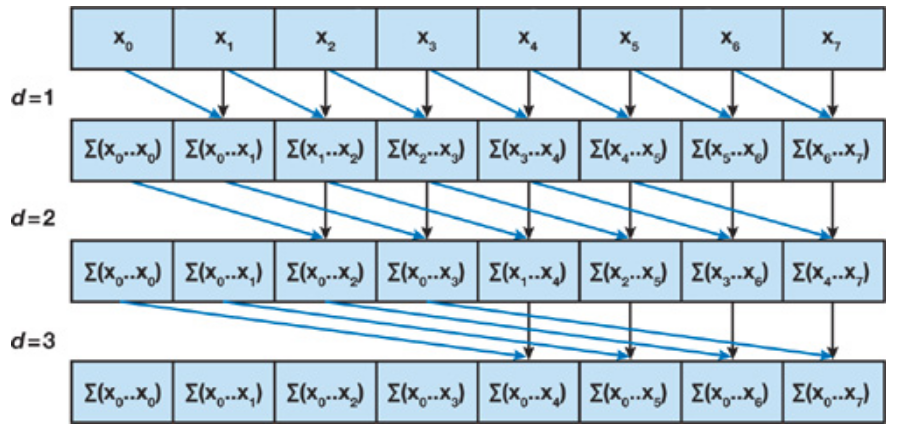
\includegraphics[width=10cm,height=5.0cm]{Figures/naivescan.png}
		\caption{An ilustration of the algorithm proposed by Horn}
	\end{figure} 	
}

\frame{
	\frametitle{\textbf{Complexity Analysis}}
	The algorithm performs O($n$ $log_{2} n$) addition operations.
	\begin{itemize}
		\item The tree has $log_{2} n$ levels;
		\item It is performed O($n$) adds for each level;
	\end{itemize}
	Remember that a sequential scan performs O($n$) adds. Therefore, this naive implementation is not work-efficient. The factor of $log_{2}n$ can have a large effect on performance.
}

\frame{
\frametitle{\textbf{Algorithm (Proposed by Mark Harris in 2007 )}}
Based in Blelloch's Work (1990);\\
Two phases (Up-Sweep $\&$ Down-Sweep):
\begin{figure}[]
	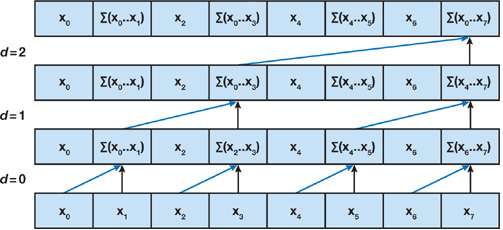
\includegraphics[width=10cm,height=5.0cm]{Figures/example_up.png}
	\caption{An illustration of the \textbf{Up-Sweep} phase}
\end{figure}
}

\frame{
	\frametitle{\textbf{An illustration of the Up-Sweep phase}}
	\begin{figure}[]
		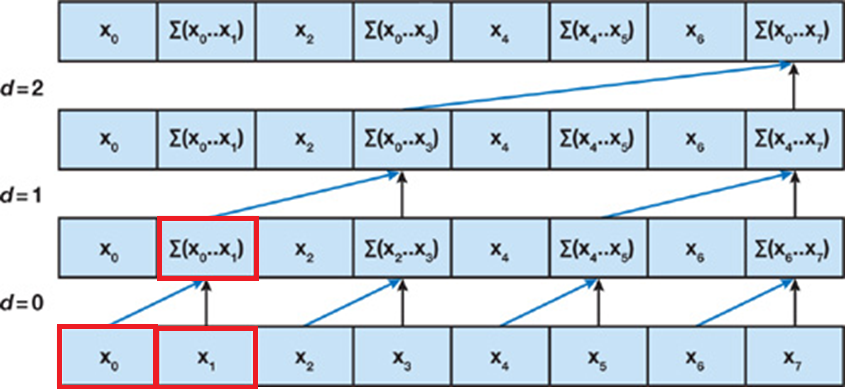
\includegraphics[width=10cm,height=5.0cm]{Figures/up1.png}
	\end{figure} 
}

\frame{
	\frametitle{\textbf{An illustration of the Up-Sweep phase}}
	\begin{figure}[]
		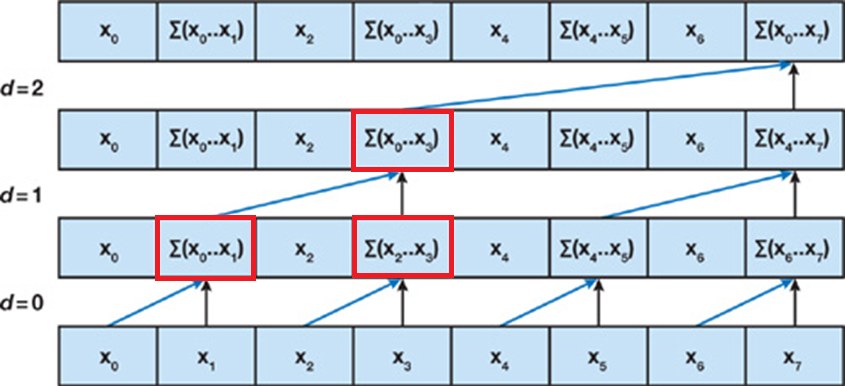
\includegraphics[width=10cm,height=5.0cm]{Figures/up2.png}
	\end{figure} 
}

\frame{
	\frametitle{\textbf{An illustration of the Up-Sweep phase}}
	\begin{figure}[]
		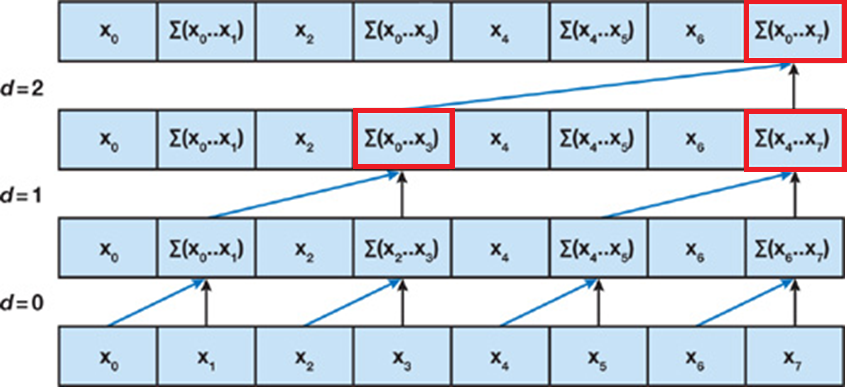
\includegraphics[width=10cm,height=5.0cm]{Figures/up3.png}
	\end{figure} 
}

\frame{
	\frametitle{\textbf{An illustration of the Down-Sweep phase}}
	\begin{figure}[]
		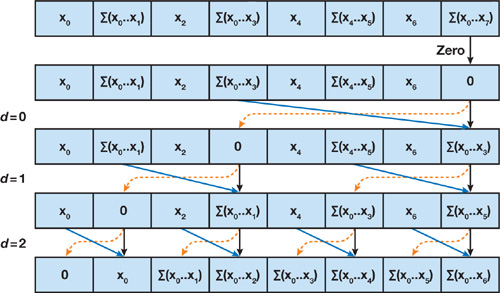
\includegraphics[width=10cm,height=5.0cm]{Figures/down.png}
	\end{figure}
}

\frame{
	\frametitle{\textbf{An illustration of the Down-Sweep phase}}
	\begin{figure}[]
		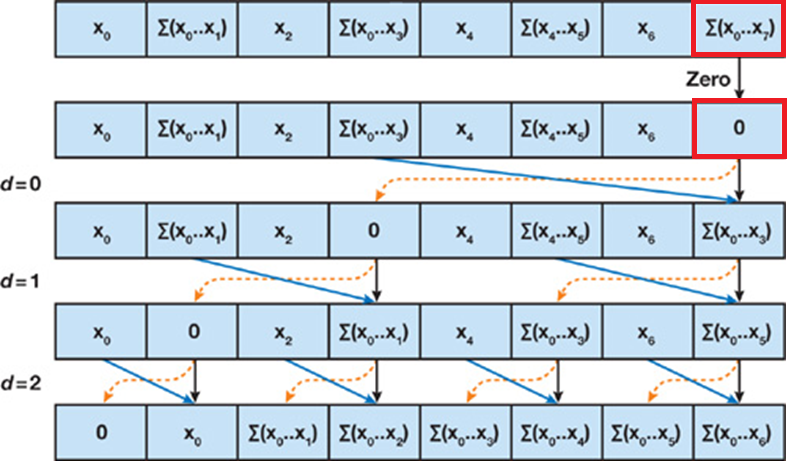
\includegraphics[width=10cm,height=5.0cm]{Figures/down1.png}
	\end{figure}
}

\frame{
	\frametitle{\textbf{An illustration of the Down-Sweep phase}}
	\begin{figure}[]
		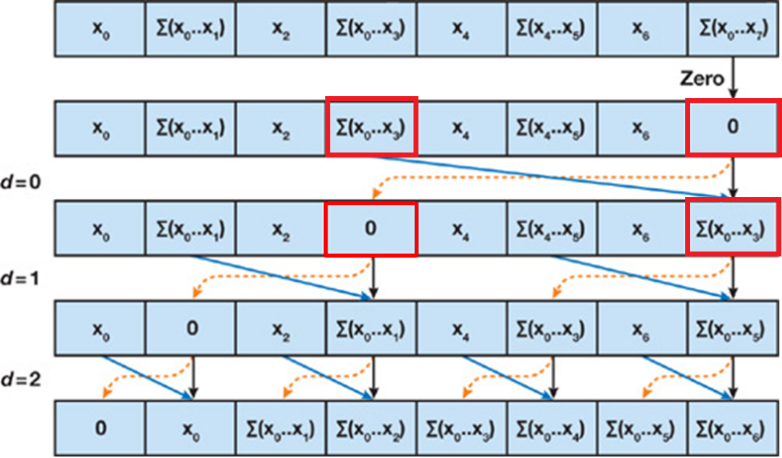
\includegraphics[width=10cm,height=5.0cm]{Figures/down3.png}
	\end{figure}
}

\frame{
	\frametitle{\textbf{An illustration of the Down-Sweep phase}}
	\begin{figure}[]
		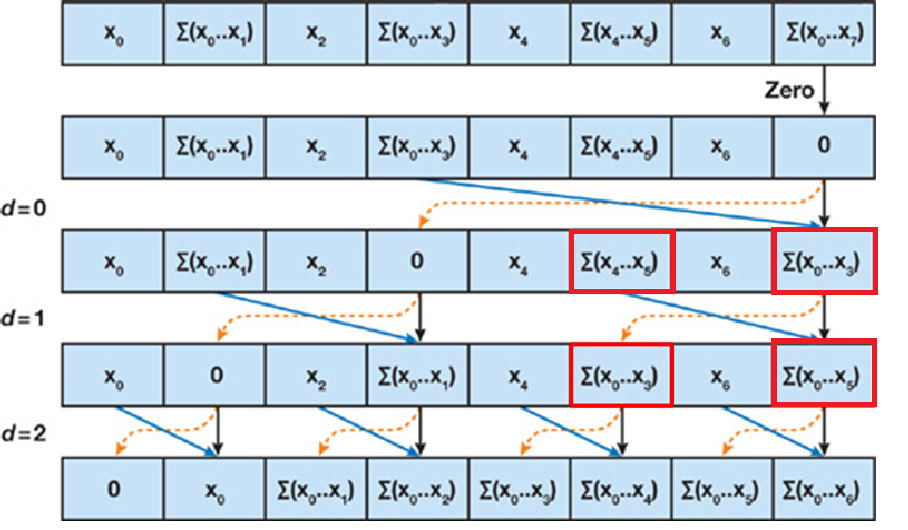
\includegraphics[width=10cm,height=5.0cm]{Figures/down4.png}
	\end{figure}
}

\frame{
	\frametitle{\textbf{An illustration of the Down-Sweep phase}}
	\begin{figure}[]
		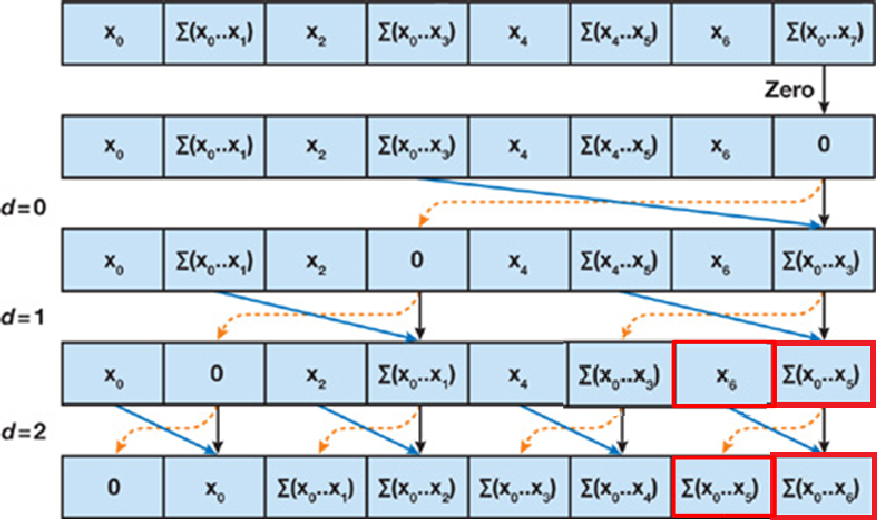
\includegraphics[width=10cm,height=5.0cm]{Figures/down5.png}
	\end{figure}
}

\frame{
	\frametitle{\textbf{Complexity Analysis}}
	Up-Sweep Complexity:
	\begin{itemize}
		\item A binary tree with $n$ leaves and $d$ = $log_{2}n$ levels, and each level $d$ has $2^{d}$ nodes. If It is performed one add per node, It is computed O(n) adds on a single traversal of the tree.
	\end{itemize}
	
	Down-Sweep Complexity:
	\begin{itemize}
		\item Similar as Up-Sweep phase. It is performed O(n) adds and O(n) swaps.
	\end{itemize}
}

\frame{
	\frametitle{\textbf{Algorithm for large arrays}}
	\begin{figure}[]
		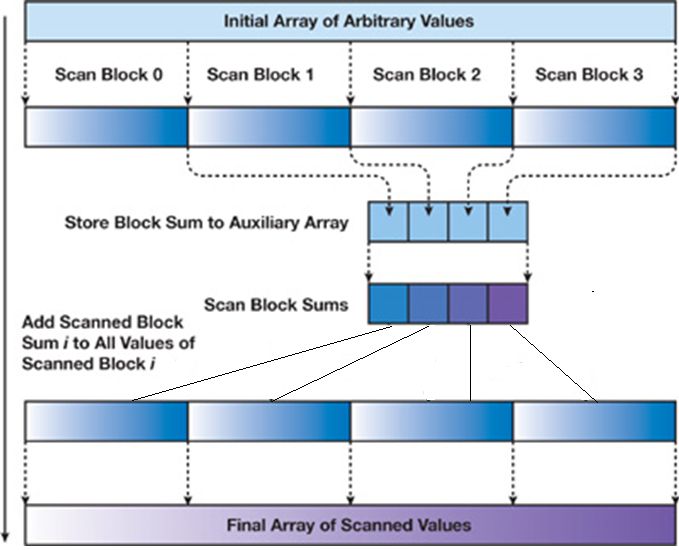
\includegraphics[width=10cm,height=7.0cm]{Figures/large.png}
	\end{figure}
}

\frame{
	\frametitle{\textbf{Algorithm for large arrays}}
	\begin{figure}[]
		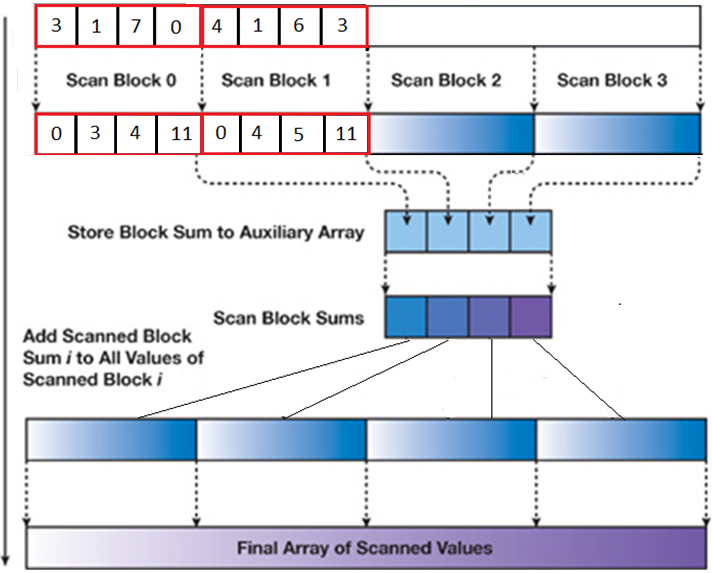
\includegraphics[width=10cm,height=7.0cm]{Figures/large1.png}
	\end{figure}
}

\frame{
	\frametitle{\textbf{Algorithm for large arrays}}
	\begin{figure}[]
		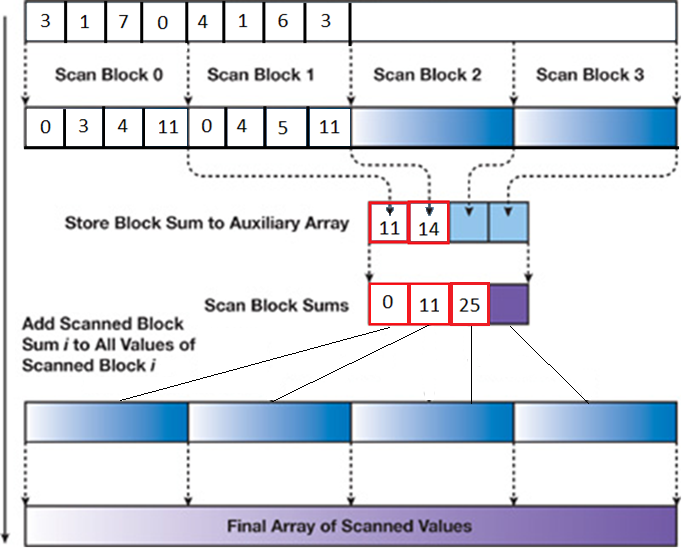
\includegraphics[width=10cm,height=7.0cm]{Figures/large2.png}
	\end{figure}
}

\frame{
	\frametitle{\textbf{Algorithm for large arrays}}
	\begin{figure}[]
		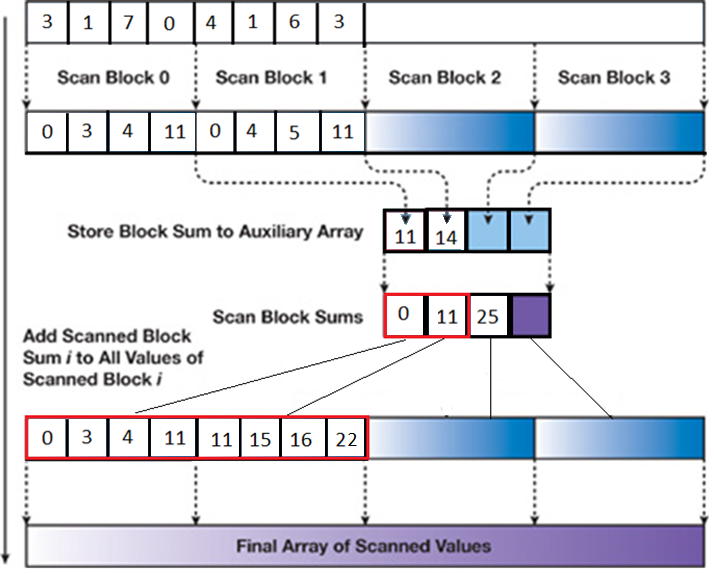
\includegraphics[width=10cm,height=7.0cm]{Figures/large3.png}
	\end{figure}
}

%------------------Scan Clause in AClang---------------------
\section{Scan Clause in AClang}
\begin{frame}
	\frametitle{\textbf{Table of Contents}}
	\tableofcontents[currentsection]
\end{frame}

\frame{
	\frametitle{\textbf{What is AClang?}}
	\begin{columns}
	\column{0.5\textwidth}
	\centering{ 
\includegraphics[width=5cm,height=4.5cm]{Figures/aclang.png} }
	\column{0.5\textwidth}
	\begin{itemize}
		\item{AClang compiler is based in LLVM Clang 3.5;}
		\item{Designed by our group at UNICAMP;}
		\item{Supports Offloading to accelerators;}
		\item{From OMP to OpenCL or SPIR code.}
	\end{itemize}
	\end{columns}	
}

\frame{
	\frametitle{\textbf{AClang Compiler Pipeline}}
	
	\begin{figure}[]
		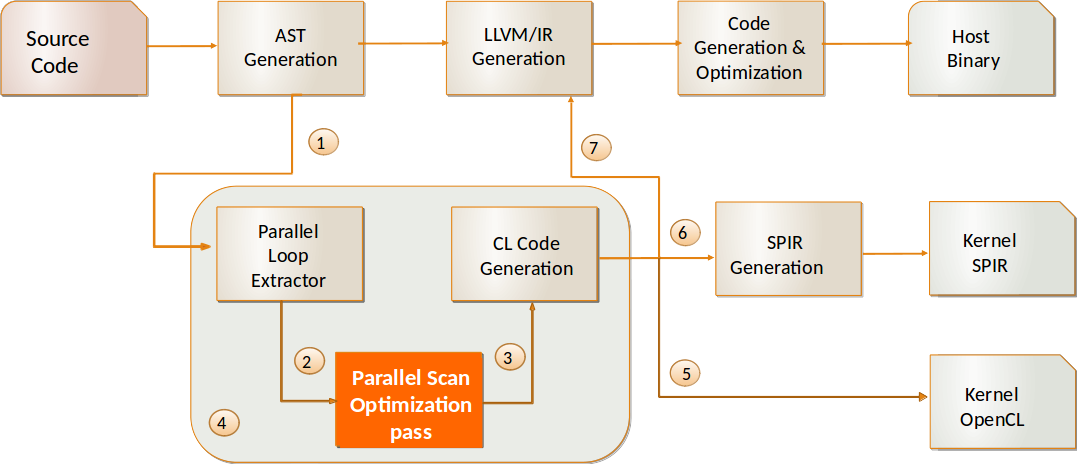
\includegraphics[width=12.30cm,height=6.7cm]{Figures/pipelineAClang.png}
	\end{figure}
}

\defverbatim[colored]\makeset{
\belowcaptionskip=-10pt
\begin{lstlisting}[language=C++,label=scanSeq,keywordstyle=\color{blue},basicstyle = \ttfamily\small,caption=Sequential Implementation of Scan]
void scan(int *x,int *y,int n) {
  y[0] = 0;
  for(i = 1; i < n; i++)
    y[i] = y[i-1] + x[i-1];
}
\end{lstlisting}
\begin{lstlisting}[language=C++,label=scanSeq,keywordstyle=\color{blue},basicstyle = \ttfamily\small,caption=Parallel implementation of Scan using the new clause]
void scan(int *x,int *y,int n) {
  y[0] = 0;
  <@\textcolor{blue}{\#pragma omp target device}@> (<@\textcolor{red}{device}@>)\
             map(to:x[:N]) map(from:y[:N])
  <@\textcolor{blue}{\#pragma omp parallel for}@> <@\textcolor{red}{scan}@> (+:y)
  for(i = 1; i < n; i++)
    y[i] = y[i-1] + x[i-1];
}
\end{lstlisting}
}

\frame{
	\frametitle{\textbf{AClang Compiler}}
	\makeset
}

\subsection{Implementation of Scan in AClang}
\begin{frame}
	\frametitle{\textbf{Table of Contents}}
	\tableofcontents[currentsection,
	currentsubsection,
	subsectionstyle=show/shaded/hide]
\end{frame}

\frame{
	\frametitle{\textbf{Implmentation of Scan in AClang}}
	The implementation is based on the best parallel scan algorithm known
	today (Mark Harris).\\
	Main steps:
	\begin{itemize}
		\item The algorithm obtains the pieces of information of the \textcolor{blue}{omp scan clause} (variable type, operator, vector size);
		\item Compute the number of blocks and threads per block to use (Scan algorithm just work for $2^{k}$ vector sizes);
		\item Generate code for the runtime library to call
		the OpenCL driver to compile the kernels and dispatch them for execution;
		\item Send information from \textcolor{blue}{omp declare target section} (new variables types and operator overload).
	\end{itemize}	
}

\subsection{The Template}
\begin{frame}
	\frametitle{\textbf{Table of Contents}}
	\tableofcontents[currentsection,
	currentsubsection,
	subsectionstyle=show/shaded/hide]
\end{frame}


\frame{
	\frametitle{\textbf{The Template}}
	The template represents the algorithm explained in the following figure:
	\begin{figure}[]
		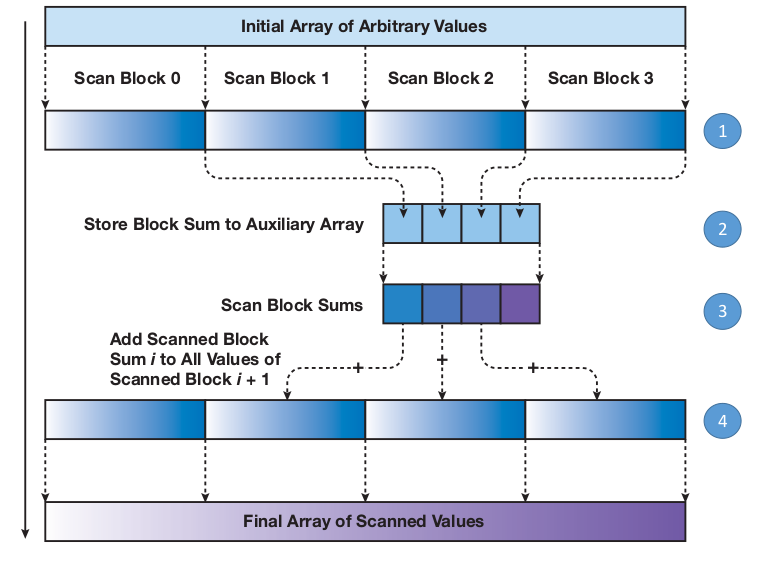
\includegraphics[width=10cm,height=7.0cm]{Figures/template.png}
	\end{figure}
}

\defverbatim[colored]\makeset{
\belowcaptionskip=-10pt
\begin{lstlisting}[language=C++,label=template,keywordstyle=\color{blue},basicstyle = \ttfamily\small,caption=Template's Structure]
//OMP_DECLARE_TARGET REGION
//END OMP_DECLARE_TARGET
#define Neutral I //Neutral value

__kernel void kernel_0 (datatype *input,\
	datatype *S, int n){
  //Performs (1) and (2)
}

__kernel void kernel_1(dataType *input, int n){
  //Performs (3)
}

__kernel void kernel_2(dataType *input,\
	 dataType *output, dataType *S){
  //Performs (4)
}

\end{lstlisting}
}

\frame{
	\frametitle{\textbf{Template's Structure}}
	\makeset 
}

\frame{
	\frametitle{\textbf{The Template}}
	The algorithm has only three parameters that could be different according to the applications.\\
	\begin{itemize}
		\item Variable type (int, float, double and so on);
		\item Operator used ($+$, $*$, $\&$, $|$, $max$, $min$ and so on);
		\item OMP declare target region (New variable type and operator).
	\end{itemize}
}

\defverbatim[colored]\makeset{
\belowcaptionskip=-10pt
\begin{lstlisting}[language=C++,label=serialtemplate,keywordstyle=\color{blue},basicstyle = \ttfamily\tiny,caption=Return the result into the input vector]

int main(){
  ...
  int aux1 = input[0], aux2;
  input[0] = 0;
  <@\textcolor{blue}{\#pragma omp target device}@> (<@\textcolor{red}{GPU}@>) map(tofrom:input[:N])
  input[0] = 0;
  <@\textcolor{blue}{\#pragma omp parallel for}@> <@\textcolor{red}{scan}@>(+:input)
  for(i = 0 ; i < n ; i++){
    aux2 = input[i];
    input[i] = input[i-1] + aux;
    aux = aux2;
  }
  ...
}

__kernel void kernel_2(dataType *input, dataType *S)

\end{lstlisting}
}

\frame{
	\frametitle{\textbf{The Template}}
	Ouput and input vector are the same. In this case the last kernel does not have the output vector, the result is overwritten in input.\\
	\makeset
}


%------------------USING THE SCAN OPERATOR---------------------
\section{Using the Scan Operator}
\begin{frame}
	\frametitle{\textbf{Table of Contents}}
	\tableofcontents[currentsection]
\end{frame}

\frame{
	\frametitle{\textbf{Example of Applications}}
	\begin{itemize}
		\item Random number generation
		\item Sequence alignment
		\item N-body problem
		\item To perform lexical analysis
		\item Polynomial Evaluation
		\item To implement Parallel Quick Sort version
		\item Array Filter
		\item Solving linear recurrences
	\end{itemize}	
}

\frame{
	\frametitle{\textbf{Example of Applications}}
	\begin{itemize}
		\item Random number generation
		\item Sequence alignment
		\item N-body problem
		\item To perform lexical analysis
		\item Polynomial Evaluation
		\item To implement Parallel Quick Sort version
		\item \color{red}{Array Filter}
		\item \color{black}{Solving linear recurrences}
	\end{itemize}	
}

\frame{
	\frametitle{\textbf{Example: Array Filter}}
	\textbf{Input}: An array A[$l$:$r$] of integers elements, and an element \textbf{x} from A[$l$:$r$].
	\textbf{Output}: Rearrange the elements of A[$l$:$r$], such that for some index $k$ $\in$ [$l$,$r$], all elements in A[$l$:$k-1$] are smaller than \textbf{x} and all elements in A[$k + 1$:$r$] are larger than \textbf{x}.
	\begin{figure}[]
		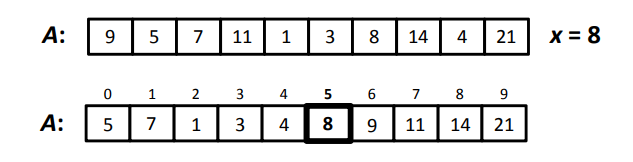
\includegraphics[width=8cm,height=2.5cm]{Figures/filter.png}
	\end{figure}
}

\frame{
	\frametitle{\textbf{Example: Array Filter}}
	\begin{figure}[]
		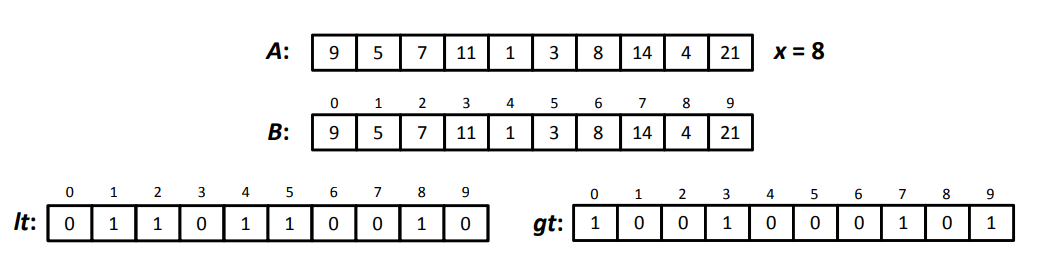
\includegraphics[width=10cm,height=3.0cm]{Figures/filter1.png}
	\end{figure}	
}

\frame{
	\frametitle{\textbf{Example: Array Filter}}
	\begin{figure}[]
		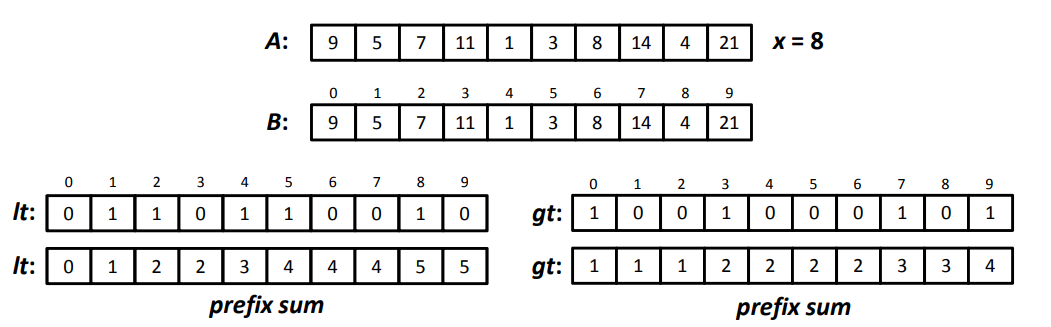
\includegraphics[width=10cm,height=4.0cm]{Figures/filter2.png}
	\end{figure}	
}

\frame{
	\frametitle{\textbf{Example: Array Filter}}
	\begin{figure}[]
		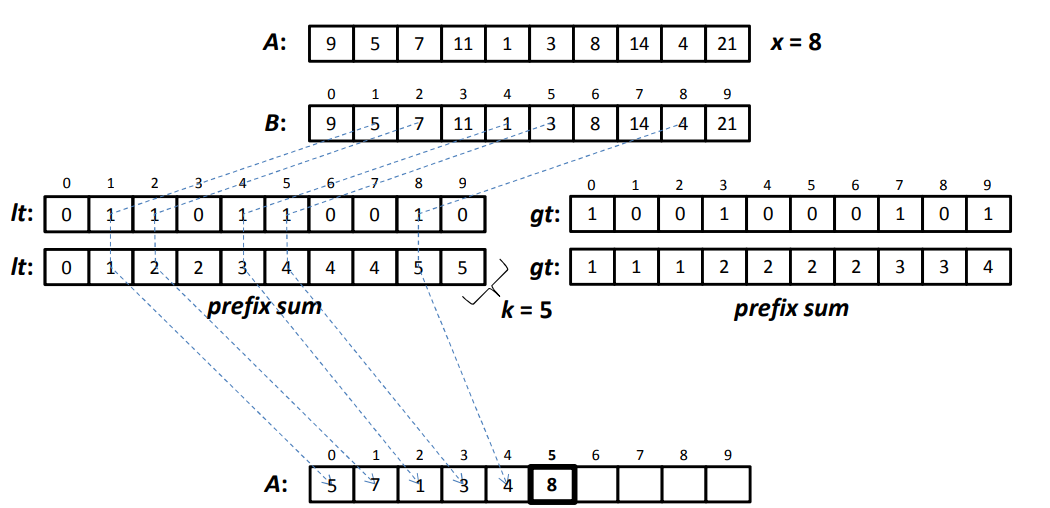
\includegraphics[width=10cm,height=5.0cm]{Figures/filter3.png}
	\end{figure}	
}

\frame{
	\frametitle{\textbf{Example: Array Filter}}
	\begin{figure}[]
		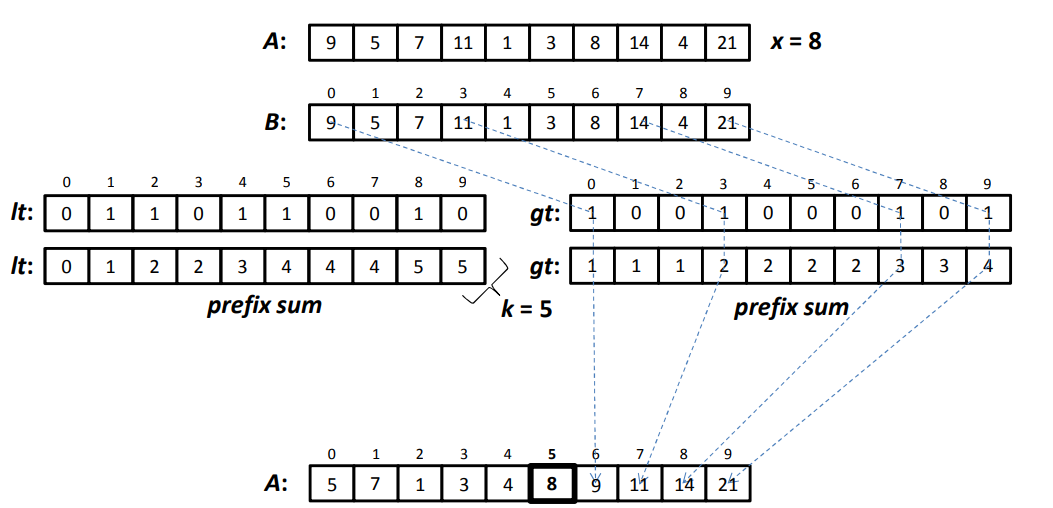
\includegraphics[width=10cm,height=5.0cm]{Figures/filter4.png}
	\end{figure}	
}

\defverbatim[colored]\makeset{
\belowcaptionskip=-10pt
\begin{lstlisting}[language=C++,label=Fibo2,keywordstyle=\color{blue},basicstyle = \ttfamily\tiny,breaklines=true,caption=Array Filter Implementation]
int main(){
  int *A, *lt , *gt, ltScan, gtScan, x, N;	
  Reading <@\textcolor{black}{and}@> allocating variables
  
  compute(lt, x, lower_equal); //In parallel
  compute(gt, x, greater);     //In parallel

  <@\textcolor{blue}{\#pragma omp target device}@> (<@\textcolor{red}{GPU}@>) map(to:lt[:N]) map(from:ltScan[:N])
  ltScan[0] = 0;
  <@\textcolor{blue}{\#pragma omp parallel for}@> <@\textcolor{red}{scan}@>(+:ltScan)
  for(i = 1 ; i < N ; i++)
    ltScan[i] = ltScan[i-1] + lt[i-1];

  <@\textcolor{blue}{\#pragma omp target device}@> (<@\textcolor{red}{GPU}@>) map(to:gt[:N]) map(from:gtScan[:N])
  gtScan[0] = 0;
  <@\textcolor{blue}{\#pragma omp parallel for}@> <@\textcolor{red}{scan}@>(+:gtScan)
  for(i = 1 ; i < N ; i++)
    gtScan[i] = gtScan[i-1] + gt[i-1];

  Rearrange the elements from A, <@\textcolor{black}{using}@> lt, gt, ltScan <@\textcolor{black}{and}@> gtScan //In parallel
}
\end{lstlisting}
}

\frame{
	\frametitle{\textbf{Source Code: Array Filter}}
	\makeset	
}

\defverbatim[colored]\makeset{
\belowcaptionskip=-10pt
\begin{lstlisting}[language=C++,label=Fibo3,keywordstyle=\color{blue},basicstyle = \ttfamily\small,breaklines=true,caption=Array Filter Template Generated]
#define Neutral 0

__kernel void kernel_0 (__global int *input,\
                        __global int *S, const int n)
                        
__kernel void kernel_1 ( ... )

__kernel void kernel_2 ( ... )

\end{lstlisting}
}

\frame{
	\frametitle{\textbf{Source Code: Array Filter}}
	\makeset	
}

\frame{
	\frametitle{\textbf{Example of Applications}}
	\begin{itemize}
		\item Random number generation
		\item Sequence alignment
		\item N-body problem
		\item To perform lexical analysis
		\item Polynomial Evaluation
		\item To implement Parallel Quick Sort version
		\item Array Filter
		\item \color{red}{Solving linear recurrences}
	\end{itemize}	
}

\defverbatim[colored]\makeset{
	\belowcaptionskip=-10pt
	\begin{lstlisting}[language=C++,label=Fibo2,keywordstyle=\color{blue},basicstyle = \ttfamily\tiny,breaklines=true,caption=Fibonacci Implementation]
<@\textcolor{blue}{\#pragma omp declare target}@>
struct Matrix{
	long x00. x01, x10, x11;
	//Default constructor
	Matrix(){
		x00 = 1; x01 = 1;
		x10 = 1; x11 = 1;
	}
};

Matrix Operator *(Matrix A, Matrix C){
	return A*C;
}
	
<@\textcolor{blue}{\#pragma omp declare target}@>
	\end{lstlisting}
}

\frame{
	\frametitle{\textbf{A realistic Example: Fibonacci Series}}
	\begin{columns}
		\footnotesize
		\column{0.60\textwidth}
		%\centering{ 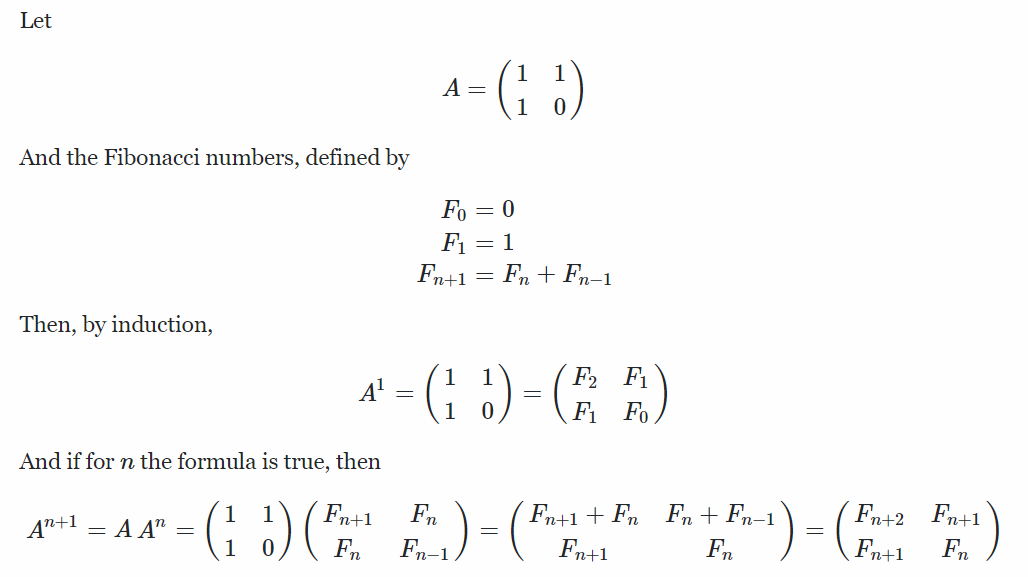
\includegraphics[width=4cm,height=3.5cm]{Figures/fibo.png} }
		\hspace*{0.5cm} Let
		\begin{align*}
		A = 
		\begin{bmatrix}
		1 & 1\\
		1 & 0
		\end{bmatrix}
		\end{align*}
		\hspace*{0.5cm} And the Fibonnacci numbers, defined by\\
		\centering $F_{0}$ = 0\\
		\centering $F_{1}$ = 1\\
		\centering $F_{n+1}$ = $F_{n}$ + $F_{n-1}$\\
		\justify \hspace*{0.5cm} Then by induction
		\begin{align*}
		A^{1} = 
		\begin{bmatrix}
		1 & 1\\
		1 & 0
		\end{bmatrix}
		=
		\begin{bmatrix}
		F_{2} & F_{1}\\
		F_{1} & F_{0}
		\end{bmatrix}
		\end{align*}
		\hspace*{0.5cm} And if for $n$ the formula is true, then:
		\begin{align*}
		A^{n+1} = A.A^{n} = 
		\begin{bmatrix}
		1 & 1\\
		1 & 0
		\end{bmatrix}
		\begin{bmatrix}
		F_{n+1} & F_{n}\\
		F_{n} & F_{n-1}
		\end{bmatrix}
		\end{align*}
		\begin{align*}
		A^{n+1} =
		\begin{bmatrix}
		F_{n+1} + F_{n} & F_{n} + F_{n-1}\\
		F_{n+1} & F_{n}
		\end{bmatrix}
		=
		\begin{bmatrix}
		F_{n+2} & F_{n+1}\\
		F_{n+1} & F_{n}
		\end{bmatrix}
		\end{align*}
				
		\column{0.40\textwidth}		
		\begin{figure}[h]
			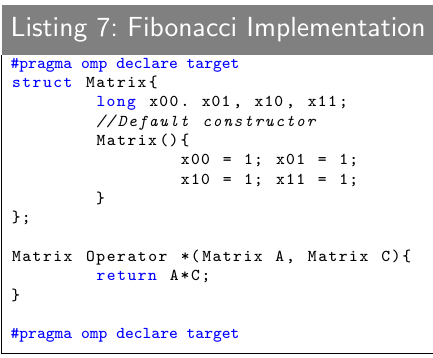
\includegraphics[width=5cm,height=4.5cm]{Figures/declare_target.png}
			%\makeset
		\end{figure}
	\end{columns}
	
}

\defverbatim[colored]\makeset{
\belowcaptionskip=-10pt
\begin{lstlisting}[language=C++,label=Fibo2,keywordstyle=\color{blue},basicstyle = \ttfamily,breaklines=true,caption=Fibonacci Implementation]
int main ( ) { 
  Matrix *x = new Matrix[N];
  Matrix *y = new Matrix[N];
  ...
  <@\textcolor{blue}{\#pragma omp target device}@> (<@\textcolor{red}{GPU}@>) \
            map (to: x[:N])  map (from: y[:N])
  y[0] = Identity_Matrix;
  <@\textcolor{blue}{\#pragma omp parallel for}@> <@\textcolor{red}{scan}@>(*:y)
  for (i = 1; i < N; i++)
    y[i] = y[i - 1] * x[i - 1];

  ...
}
\end{lstlisting}
}

\frame{
	\frametitle{\textbf{Source Code : Fibonacci Series}}
	\makeset	
}

\defverbatim[colored]\makeset{
\belowcaptionskip=-10pt

\begin{lstlisting}[language=C++,label=Fibo3,keywordstyle=\color{blue},basicstyle = \ttfamily\small,breaklines=true,caption=Fibonacci Template Generated]
struct Matrix {
  long x00, x01, x10, x11;
};
Matrix *(Matrix A, Matrix C) {
  Mat X;
  X.x00 = A.x00 * C.x00 + A.x01 * C.x10;
  X.x01 = A.x00 * C.x01 + A.x01 * C.x11;
  X.x10 = A.x10 * C.x00 + A.x11 * C.x10;
  X.x11 = A.x10 * C.x01 + A.x11 * C.x11;
  return X;
}
#define Neutral (Matrix){ 1, 0, 0, 1 }

__kernel void kernel_0 (__global Matrix *input,__global Matrix *S, const int n) 
__kernel void kernel_1 ( ... )
__kernel void kernel_2 ( ... )
\end{lstlisting}
}

\frame{
	\frametitle{\textbf{Source Code : Fibonacci Series}}
	\makeset	
}

\frame{
	\frametitle{\textbf{Source Code : Fibonacci Series}}
	\begin{figure}[]
		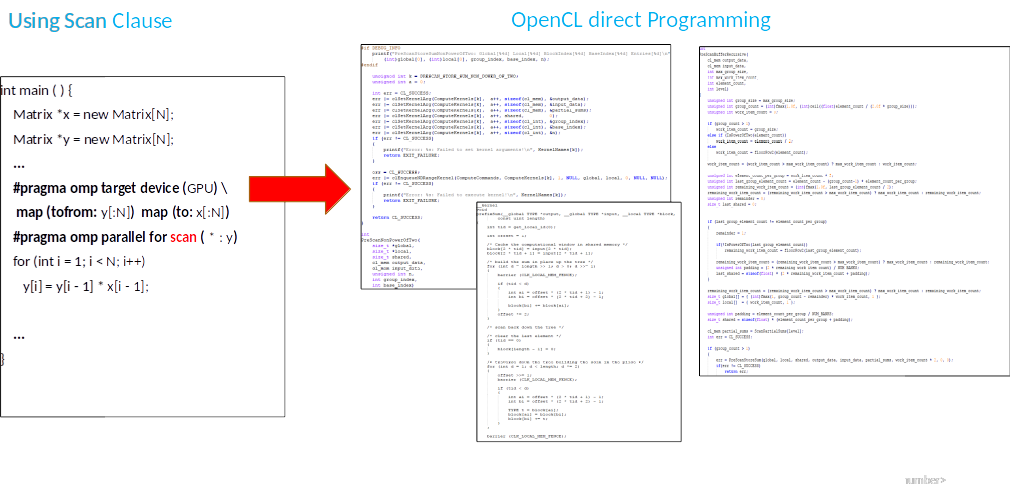
\includegraphics[width=12.3cm,height=6.8cm]{Figures/passto.png}
	\end{figure}
}

%-----------------Experimental Evaluation---------------------

\section{Experimental Evaluation}
\begin{frame}
	\frametitle{\textbf{Table of Contents}}
	\tableofcontents[currentsection]
\end{frame}

\frame{
	\frametitle{\textbf{a) The execution on Intel Xeon CPU E5-2620 with NVIDIA Tesla K40c}}
	\begin{figure}[]
		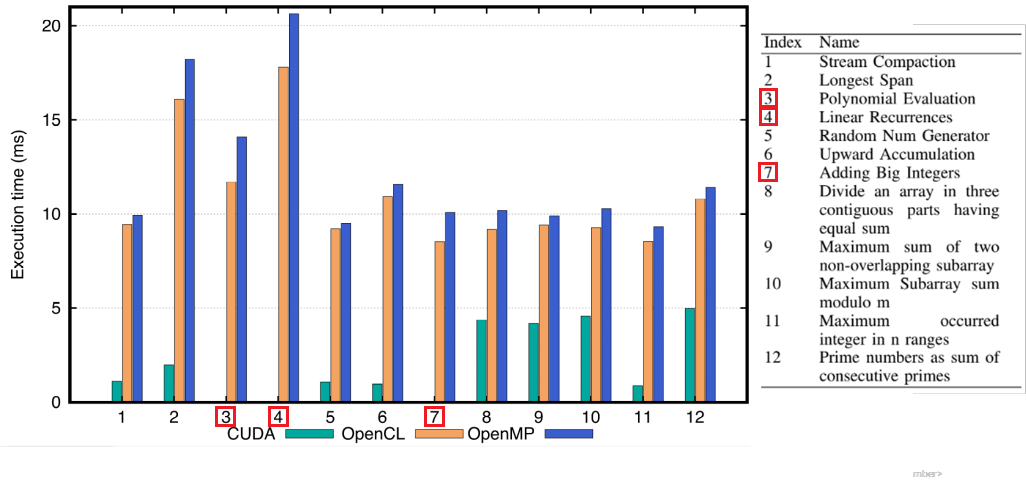
\includegraphics[width=12.3cm,height=6.5cm]{Figures/resul1.png}
	\end{figure}
}

\frame{
	\frametitle{\textbf{b) The execution on Intel Core i5 with Intel Iris GPU}}
	\begin{figure}[]
		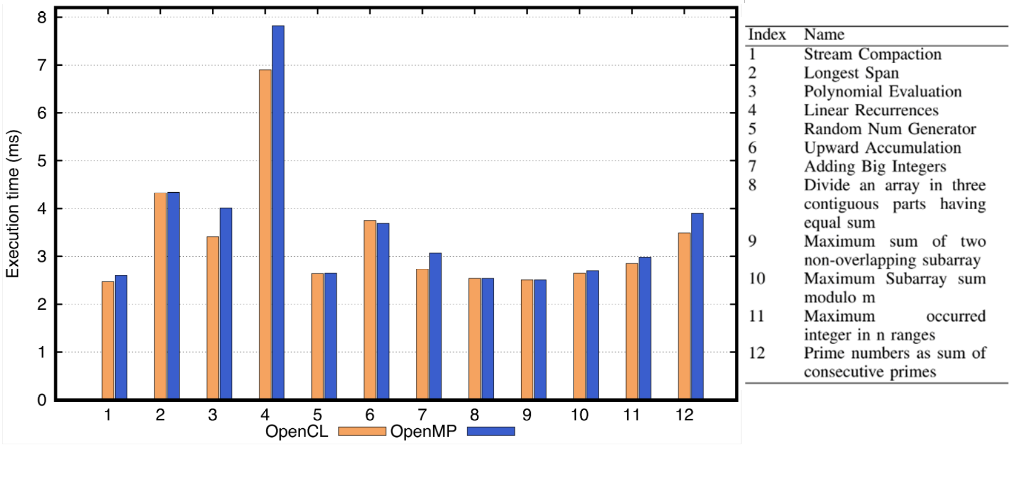
\includegraphics[width=12.3cm,height=6.5cm]{Figures/resul2.png}
	\end{figure}
}

%*******************Conclusion and Future Works*******************
\section{Conclusion and Future Works}
\begin{frame}
	\frametitle{\textbf{Table of Contents}}
	\tableofcontents[currentsection]
\end{frame}

\frame{
	\frametitle{\textbf{Conclusion and Future Works}}
	Conclusion:
	\begin{itemize}
		\item The scan operation is a simple  and powerful parallel primitive with a
		broad  range  of  applications;
		\item The new scan clause in OpenMP exhibits a similar performance as direct programming in OpenCL at a much smaller design effort.
	\end{itemize}	
	
	
}

\frame{
	\frametitle{\textbf{Conclusion and Future Works}}
	Future Works:
	\begin{itemize}
		\item Implement a template of scan algorithm for NVIDIA;
		\item Extend the limits of scan;
		\item Implement a template of reduction algorithm for AClang compiler;
		\item Improve the scan clause the performance by
		providing specific routines to handle scan operations
		into the AClang  runtime  library.
	\end{itemize}
}

\frame{
	\frametitle{\textbf{Thanks}}
	\begin{figure}[!htbp]
		
\includegraphics[scale=0.4]{Figures/thanks.png}
	\end{figure} 
	\hspace*{9.0cm} 
\includegraphics[scale=0.2]{Figures/capes.png} 
}

\end{document} \grid
